\chapter{Предложенный алгоритм и исследование его свойств}

% Предлагается рассмотреть другой подход к оценке параметра положения и матрицы разброса, отличный от упомянутых методов, основанных на подборе незагрязненных выбросами подвыборок и/или перебирающими аттракторы.

\section{Предложенный алгоритм оценки параметра положения}

Ранее был предложен и исследован~\cite{filatova2024robust} Алгоритм \ref{alg:median}, который рассматривался как метод оценки центра симметрии. Величина, которая получается в результате работы алгоритма --- \textbf{стохастическая медиана}.

\begin{algorithm}[H]
\caption{Вычисление оценки некоторого обобщения многомерной медианы}
\begin{algorithmic}[1]
			\State Рассматриваем выборку $\mathbf{x}_1,\ldots,\mathbf{x}_{{n}}$. 
			\State Произвольным образом выбираем точку $\widehat{\mathbf{m}}_1$ --- начальное приближение медианы. Задаем критерий останова. $i=1$ --- первый шаг алгоритма. 
			\State Рассматриваем случайный вектор $\mathbf{u}_i$, равномерно распределенный на единичной сфере. Проводим прямую 
			\[l_{\text{i}}=\{\widehat{\mathbf{m}}_{{i}}+\lambda\mathbf{u}_{{i}},\;\lambda\in\mathbb{R}\}.\]
			\State Проектируем наблюдения $\mathbf{x}_1,\ldots,\mathbf{x}_{{n}}$ на эту прямую, получаем точки-проекции~$y_{i1},\ldots,y_{in}$.
			\State Находим медиану $\widehat{\mathbf{m}}_{{i+1}}$ точек $y_{{i1}},\ldots,y_{{in}}$. 
			\State Алгоритм завершается, когда выполняется критерий останова, например,  $\|\widehat{\mathbf{m}}_{{i}}-\widehat{\mathbf{m}}_{{i+1}}\|<\varepsilon$.  Иначе увеличиваем $i$ на 1 и возвращаемся к шагу 3.
\end{algorithmic}
\label{alg:median}
\end{algorithm}

\section{Эквивалентность проекционной медиане}

На первый взгляд Алгоритм \ref{alg:median} представляет собой эвристическую итеративную процедуру, использующую случайные направления и одномерные медианы проекций. Однако возникает естественный вопрос о том, существует ли функционал, минимизацию которого фактически реализует данный алгоритм.

Для ответа на этот вопрос рассмотрим связь предложенного алгоритма с методом yamm и классическим методом стохастического градиента.

\vspace{1ex}

\textbf{Классический метод стохастического градиента с фиксированной длиной шага}

Рассмотрим целевую функцию следующего вида: $g(\boldsymbol{x}) = \mathrm{E} f(\boldsymbol{x}, \boldsymbol{\xi})$, где $\boldsymbol{\xi}$ имеет распределение $\Xi$.  Для решения оптимизационной задачи
\begin{equation}\label{eq:stochast_grad}
\boldsymbol{x}^* = \arg\min_{\boldsymbol{x}} g(\boldsymbol{x}).
\end{equation}
применяется \emph{метод стохастического градиента} \cite{RobbinsMonro1951}:

\begin{algorithm}[H]
\caption{Метод стохастического градиента}
\begin{algorithmic}[1]
    \State Положим $\boldsymbol{x}_0$ --- начальное приближение.
    \State Пока не выполнено условие остановки, выполняем:
        \item[] \hspace{\algorithmicindent} a) Моделируем независимую $\boldsymbol{\xi}_i$ из $\Xi$.
        \item[] \hspace{\algorithmicindent} b) Считаем $\nabla_{\boldsymbol{x}} f(\boldsymbol{x}_i, \boldsymbol{\xi}_i)$ --- градиент в точке $\boldsymbol{x}_i$ по $\boldsymbol{x}$.
        \item[] \hspace{\algorithmicindent} c) Вычисляем новое приближение:
        \begin{equation}\label{eq:sg_it}
        \boldsymbol{x}_{i+1} =\boldsymbol{x}_i - \alpha \nabla_{\boldsymbol{x}} f(\boldsymbol{x}_i, \boldsymbol{\xi}_i),
        \end{equation}
        \item[] \hspace{\algorithmicindent} \phantom{c)} где $\alpha$ --- длина шага, $i = i + 1$.
\end{algorithmic}
\label{alg:stochgrad}
\end{algorithm}

Обычно $\Xi$ имеет эмпирическое (дискретное) распределение, и шаг моделирования $\boldsymbol{\xi}_i$ интерпретируется как случайный выбор элемента из исходной выборки. Однако в рассматриваемой задаче такой подход не подходит, поскольку в качестве распределения $\Xi$ требуется использовать непрерывное распределение на единичной сфере.

\vspace{1ex}

\textbf{Основное утверждение}

Пусть $\boldsymbol{\omega}$ --- случайная величина, равномерно распределенная на единичной сфере $\Omega_d$. Тогда целевую функцию метода yamm \eqref{eq:yamm_tf} можно записать в эквивалентном (с точностью до константы $c$) виде:
\begin{equation}\label{eq:stochast_tf}
N_{\mathbf{X}}(\boldsymbol{\mu}) = \mathrm{E}_{\boldsymbol{\omega}} m_{\mathbf{X}} (\boldsymbol{ \mu}, \boldsymbol{ \omega})^2,
\end{equation}
то есть, $N_{\mathbf{X}}(\boldsymbol{\mu}) = c M_{\mathbf{X}}(\boldsymbol{\mu})$.

Для доказательства основного результата потребуется следующее вспомогательное утверждение, его доказательство непосредственно следует из определения одномерной медианы.
\begin{proposition}
Пусть $\mathbf{X}$ --- одномерная конечная выборка, $a + \mathbf{X}$ --- сдвиг всех точек выборки на $a \in \mathbb{R}$, $m(\mathbf{X})$ --- строго (однозначно) определенная медиана. Тогда $m(a + \mathbf{X}) = a + m(\mathbf{X})$, $\left(m(a + \mathbf{X}) \right)'_a = 1$.
\end{proposition}

\begin{theorem}\label{eq:thetheorem}
Алгоритм \ref{alg:median} является методом стохастического градиента (Алгоритм \ref{alg:stochgrad}) для оптимизации целевой функции \eqref{eq:stochast_tf} с длиной шага $\alpha = 0{,}5$.
\end{theorem}

\begin{proof}
\small
Заметим, что целевая функция $N_{\mathbf{X}}(\boldsymbol{\mu})$ \eqref{eq:stochast_tf} удовлетворяет виду $g(\boldsymbol{x})$ из \eqref{eq:stochast_grad} для $\boldsymbol{x}:=\boldsymbol{\mu}$.


Покажем, что шаг Алгоритма \ref{alg:median} совпадает с шагом метода стохастического градиента. Для этого вычислим градиент функции, стоящей под знаком математического ожидания в \eqref{eq:stochast_tf}, по переменной $\boldsymbol{x}:=\boldsymbol{\mu}$:
\begin{equation*}
\nabla_{\boldsymbol{x}} m_{\mathbf{X}}(\boldsymbol{x}, \boldsymbol{\omega})^2 = 2 m_{\mathbf{X}} (\boldsymbol{x}, \boldsymbol{\omega}) \nabla_{\boldsymbol{x}} m_{\mathbf{X}}(\boldsymbol{x}, \boldsymbol{\omega}) = -2m_{\mathbf{X}} (\boldsymbol{x}, \boldsymbol{\omega})\boldsymbol{\omega}.
\end{equation*}

Подставим полученное выражение в формулу шага \eqref{eq:sg_it} при $\alpha = \frac{1}{2}$:
\begin{equation*}
    \boldsymbol{x}_{i+1} = \boldsymbol{x}_i + \frac 1 2 \cdot 2 m_{\mathbf{X}} (\boldsymbol{x}_i, \boldsymbol{\omega}_i) \boldsymbol{\omega}_i = \boldsymbol{x}_i + m_{\mathbf{X}} (\boldsymbol{x}_i, \boldsymbol{\omega}_i) \boldsymbol{\omega}_i, \ \text{где $\boldsymbol{\omega}_i = \boldsymbol{\xi}_i$, $\Xi = \Omega_d$. }
\end{equation*}
Полученный шаг совпадает с шагом 4 Алгоритма \ref{alg:median} при замене $\boldsymbol{x}_i$ на $\widehat{\mathbf{m}}_{i}$, $\boldsymbol{\omega}_i$ на $\mathbf{u}_i$.
\end{proof}


Теорема \ref{eq:thetheorem} показывает, что предложенный алгоритм можно интерпретировать не просто как эвристическую процедуру, а как стохастический метод оптимизации функционала, связанного с проекционной медианой. Следовательно, при сходимости Алгоритма \ref{alg:median} к глобальному минимуму функции \eqref{eq:stochast_tf}, полученная оценка (стохастическая медиана) должна наследовать свойства проекционной медианы и оценки yamm, в частности робастность и эквивариантность относительно вращений.

Это позволяет использовать результаты, известные для метода yamm и проекционной медианы, при дальнейшем исследовании свойств предложенного алгоритма. В частности, возникает естественный вопрос о том, в какой степени алгоритм наследует свойства эквивариантности, поскольку его робастность уже исследовалась ранее в работе~\cite{filatova2024robust}.

\section{Проверка эквивариантности алгоритма}

Эквивариантность --- одно из желаемых свойств для алгоритмов оценки параметра положения. Напомним, что алгоритм называется аффинно-эквивариантным, если при аффинном преобразовании данных оценка изменяется согласованным образом. То есть для выборки $\mathbf{X}\in \mathbb{R}^{n\times d}$ и аффинно--преобразованых данных $\mathbf{Z}$, вычисленных по формуле \eqref{eq:affine_transform}, выполняется соотношение \eqref{eq:affine_eq_t} для некоторой оценки параметра положения $T( \mathbf{X}) \in \mathbb{R}^d$.

Стохастические алгоритмы принципиально не могут быть строго аффинно-эквивариантными из-за случайности получаемой оценки, однако было бы желательно, чтобы норма ошибки $\|T( \mathbf{Z}) - (\mathbf{A}T(\mathbf{X}) + \mathbf{b})\|$ была относительно мала, в идеале близка к нулю.

Проверим это свойство эмпирически на выборках из трехмерного стандартного нормального распределения, а также на выборке из трехмерного нормального распределения с нулевым математическим ожиданием и следующей ковариационной матрицей 
\begin{equation}\label{eq:experimentmatrix}
 \boldsymbol{\Sigma}= \begin{pmatrix}
2 & 0{,}95  & 0{,}95\\
0{,}95 & 4 & 0{,}95\\
0{,}95 & 0{,}95 & 8
\end{pmatrix}.
\end{equation}

В работе~\cite{filatova2024robust} было показано, что алгоритм оценки геометрической медианы является главным конкурирующим методом по отношению к предложенному алгоритму. Поэтому далее сравним ошибки эквивариантности для обоих методов. Ошибка определяется как разность между полученным алгоритмом значением $\widehat{\mathbf{m}}$ и истинным значением медианы $\mathbf{m}$.

Для проверки рассмотрим следующие типы преобразований:
\begin{itemize}
    \item Произвольную невырожденную матрицу $\mathbf{A}$;
    \item Диагональную матрицу $\mathbf{D}$, соответствующую растяжению координат;
    \item Произвольную ортогональную матрицу $\mathbf{O}$, соответствующую повороту, отражению или перестановке координат;
    \newpage
    \item Матрицу сдвига $\mathbf{S}$, которая в случае трехмерного распределения задается как
  \begin{align*}
    \begin{pmatrix}
1 \; & \lambda\;   & \nu \\
0 \; & 1 &\;  0 \\
0 \; & 0\;  & 1
\end{pmatrix}, \quad \text{где} \quad \lambda, \; \nu\in\mathbb{R}.
    \end{align*}
\end{itemize}

\begin{figure}[!hhh]
   \centering
    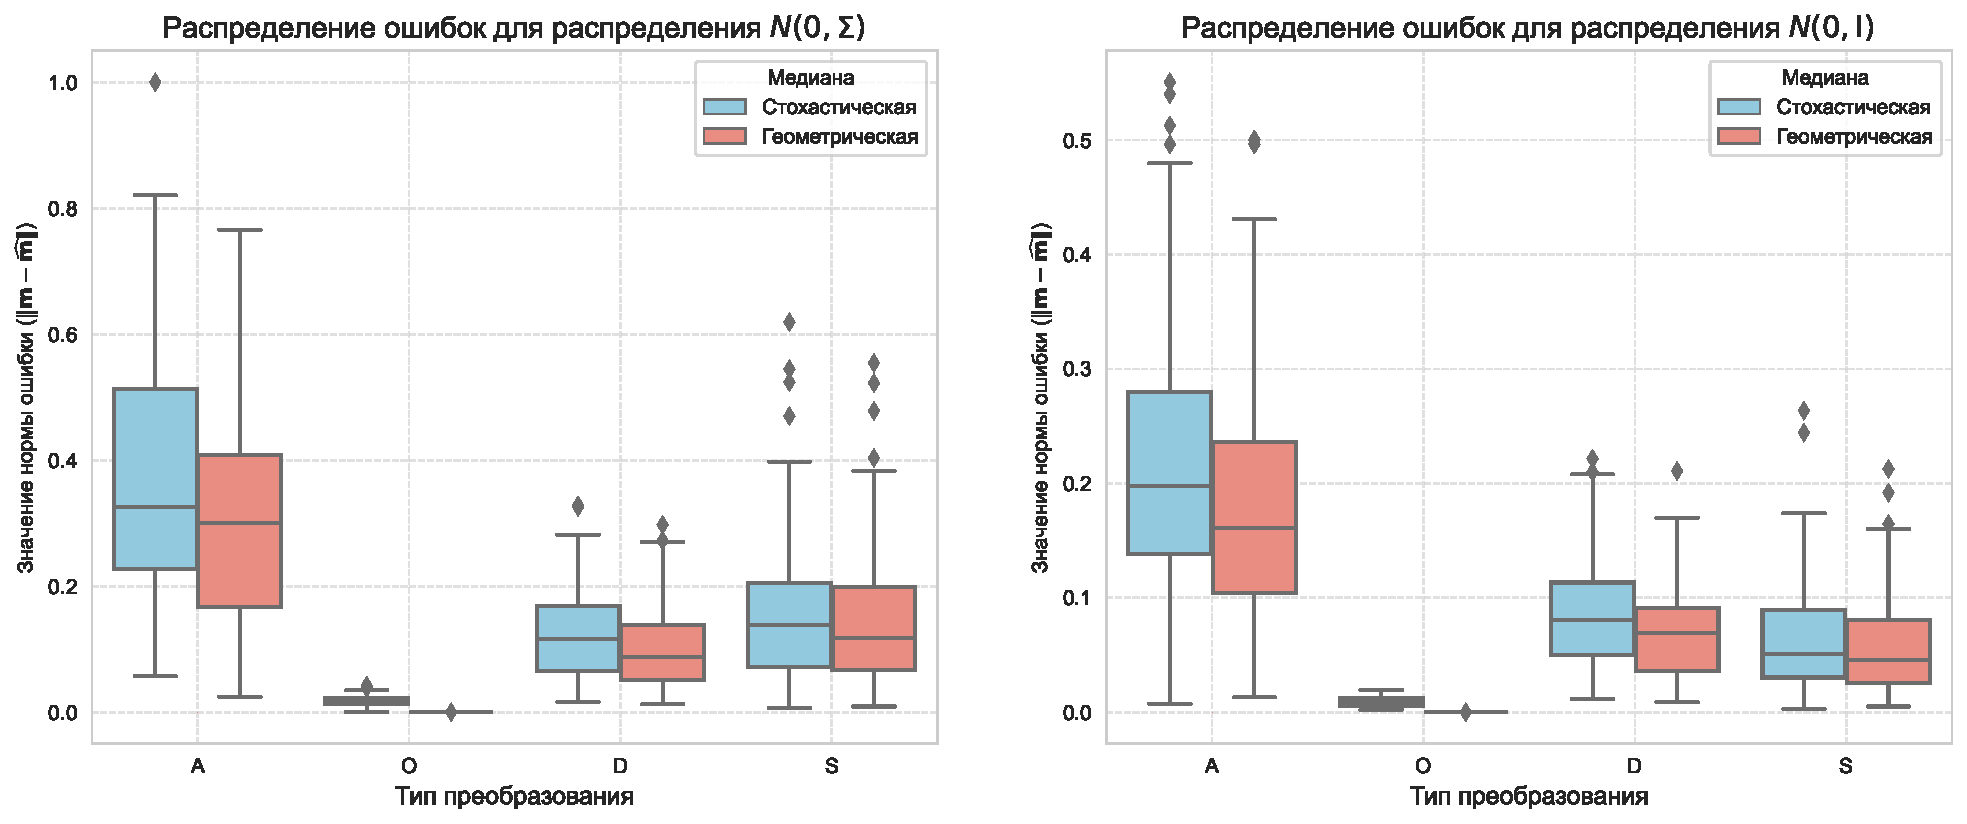
\includegraphics[width=15cm]{geom_exp_comp_equivariant.pdf}
  \caption{Сравнение распределений ошибок эквивариантности для алгоритма оценки геометрической медианы и предложенного алгоритма.}
  \label{fig:geom_exp_comp_equivariant}
\end{figure}

Результаты сравнения представлены на Рисунке~\ref{fig:geom_exp_comp_equivariant}. Видно, что для предложенного алгоритма ошибка близка к нулю только в случае ортогональных преобразований, причем данное свойство наблюдается для обоих рассматриваемых распределений. Это согласуется с результатами предыдущего раздела, где было показано, что алгоритм связан с проекционной медианой и методом yamm, обладающими эквивариантностью относительно поворотов.

Для диагональных преобразований и матриц сдвига ошибки остаются сравнительно малыми: медианные значения не превышают $0{,}1$. Однако в случае произвольных невырожденных преобразований ошибка возрастает примерно в два раза.

Для геометрической медианы наблюдается аналогичный характер поведения. При этом ошибки геометрической медианы в среднем несколько меньше, чем у предложенного алгоритма. Это указывает на необходимость дальнейшей доработки реализации стохастического алгоритма.

\section{Результаты работы алгоритма для различного вида областей и распределений}

% В предыдущих разделах были исследованы теоретические свойства предложенного алгоритма, а также его связь с проекционной медианой. Однако не менее важно понять, как алгоритм ведет себя на выборках различной природы.

% В данном разделе исследуется поведение предложенного алгоритма на выборках из непрерывных и дискретных распределений, а также в областях различной геометрии: выпуклых, невыпуклых и несвязных. 

В предыдущих разделах были исследованы теоретические свойства предложенного алгоритма и его связь с проекционной медианой. Далее рассмотрим поведение алгоритма на выборках различной природы: для непрерывных и дискретных распределений, а также в областях различной формы.

\subsection{Несвязная область}

Рассмотрим работу различных алгоритмов оценки параметра положения на выборке из равномерного распределения в несвязной области (Рисунок~\ref{fig:disjoint_1000}). Видно, что все алгоритмы, кроме медианы Оджа, дают близкие оценки, расположенные вблизи выборочного среднего. 

%Таким образом, наличие двух разделенных кластеров не оказывает существенного влияния на поведение большинства рассматриваемых методов.
\vspace{-0.5ex}

\begin{figure}[!hhh]
   \centering
    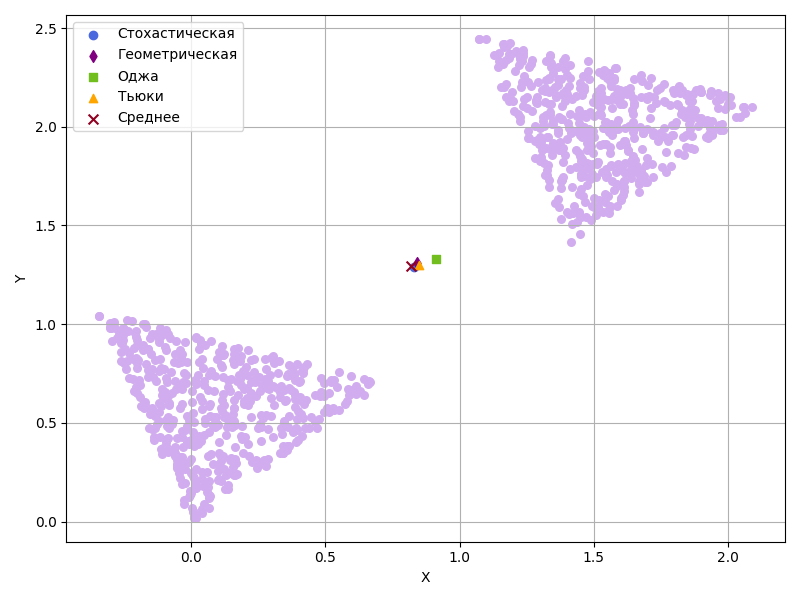
\includegraphics[width=0.95\textwidth]{sample_1000_med_and_mean.png}
  \caption{Сравнение различных оценок многомерной медианы для выборки объема 1000 из равномерного распределения в несвязной области.}
  \label{fig:disjoint_1000}
\end{figure}

\newpage

\subsection{Произвольная выпуклая область}

Далее рассмотрим выборку из равномерного распределения внутри выпуклой области (Рисунок~\ref{fig:convex}).

Как видно из рисунка, все рассматриваемые алгоритмы дают близкие оценки параметра положения, расположенные вблизи выборочного среднего. В данном случае различия между методами оказываются минимальными.


\begin{figure}[!hhh]
   \centering
    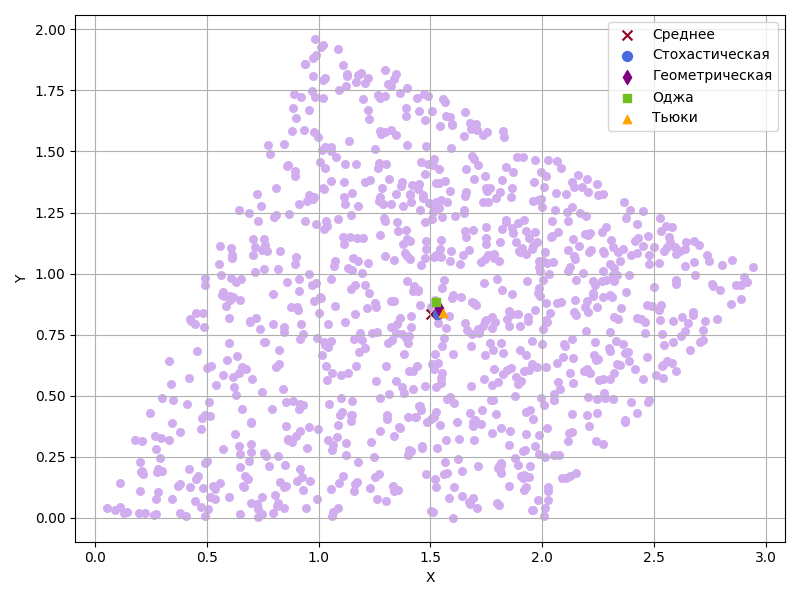
\includegraphics[width=0.95\textwidth]{sample_nonconvex.png}
  \caption{Сравнение различных оценок многомерной медианы для выборки объема 1000 из равномерного распределения в выпуклой области.} 
  \label{fig:convex}
\end{figure}
%\newpage

\subsection{Невыпуклые области}

\subsubsection{Невыпуклый пятиугольник}

Рассмотрим теперь случай равномерного распределения в невыпуклой области (Рисунок~\ref{fig:nonconvex_flag}).

Несмотря на невыпуклость области, все алгоритмы продолжают давать устойчивые оценки параметра положения, хотя наблюдается небольшое смещение относительно выборочного среднего. Это позволяет предположить, что отсутствие выпуклости у области само по себе не оказывает существенного влияния на работу рассматриваемых методов.


\begin{figure}[!hhh]
   \centering
    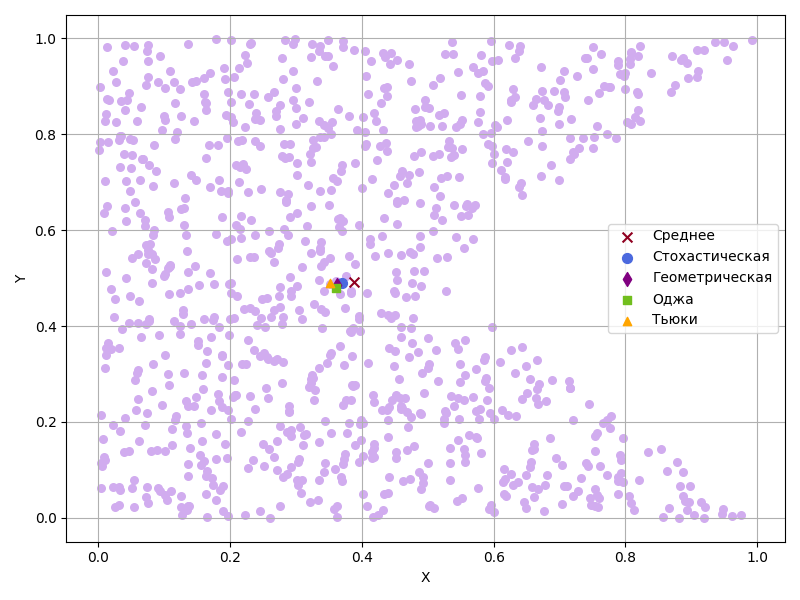
\includegraphics[width=0.95\textwidth]{sample_polygon.png}
  \caption{Сравнение различных оценок многомерной медианы для выборки объема 1000 из равномерного распределения в области в виде невыпуклого пятиугольника.
   % Сравнение различных оценок многомерной медианы для выборки объема 1000 в форме невыпуклого пятиугольника с равномерным распределением внутри области.
  }
  \label{fig:nonconvex_flag}
\end{figure}
%\newpage

\subsubsection{Кольцо}

Более интересная ситуация наблюдается в случае равномерного распределения в кольце (Рисунок~\ref{fig:ring}). Для данной выборки выборочное среднее, геометрическая медиана и медиана Тьюки дают практически совпадающие оценки, расположенные в центре области.

Предложенный алгоритм и медиана Оджа дают близкие между собой результаты, однако их оценки оказываются слегка смещенными относительно центра тяжести. Тем не менее, величина смещения остается незначительной.

\begin{figure}[!hhh]
   \centering
    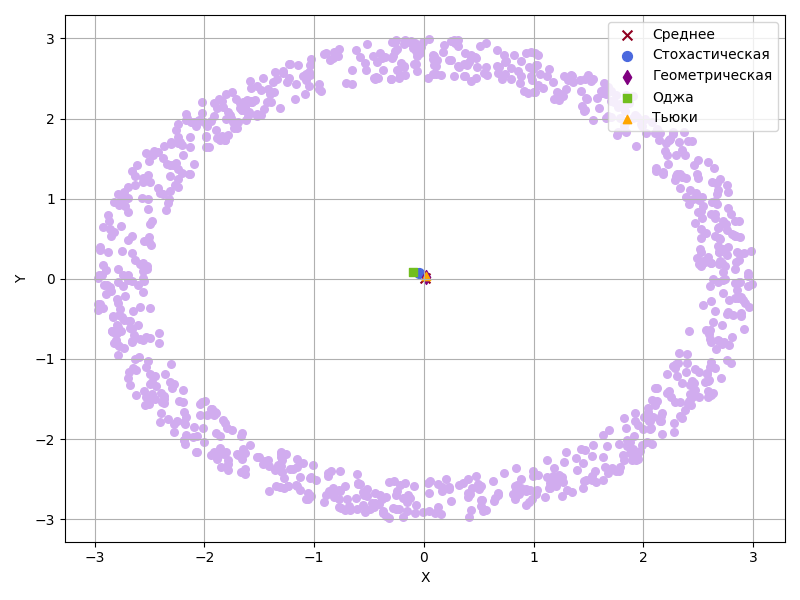
\includegraphics[width=0.95\textwidth]{sample_ring.png}
  \caption{Сравнение различных оценок многомерной медианы для выборки объема 1000 в форме кольца с равномерным распределением внутри области.}
  \label{fig:ring}
\end{figure}
\newpage

\subsection{Дискретные распределения}

Рассмотрим теперь дискретные распределения.

\vspace{-2ex}

\subsubsection{Пуассоновское двумерное}

Выборка из двумерного распределения Пуассона $X_{1},X_{2}$ получается следующим образом:  $X_{1}=Y_{1}+Y_{3},\ X_{2}=Y_{2}+Y_{3}$, где $Y_{1},Y_{2},Y_{3}$ --- независимые распределения Пуассона с параметрами $\lambda_{1},\lambda_{2},\lambda_{3}$.

Рассмотрим распределения Пуассона с параметрами $\lambda_{1} = 1,\ \lambda_{2}=2,\ $ $\lambda_{3}=3.$ Тогда параметры двумерного $\Lambda_{1}=4,\ \Lambda_{2}=5$, из чего следует, что  математическое ожидание распределения равно $(4; 5)^{\mathrm{T}}$.

Из Рисунка~\ref{fig:poisson} видно, что медианы Тьюки и Оджа, а также выборочное среднее дают практически совпадающие оценки, близкие к теоретическому математическому ожиданию. Предложенный алгоритм и геометрическая медиана также дают близкие результаты, хотя наблюдается небольшое смещение.

\begin{figure}[!hhh]
   \centering
    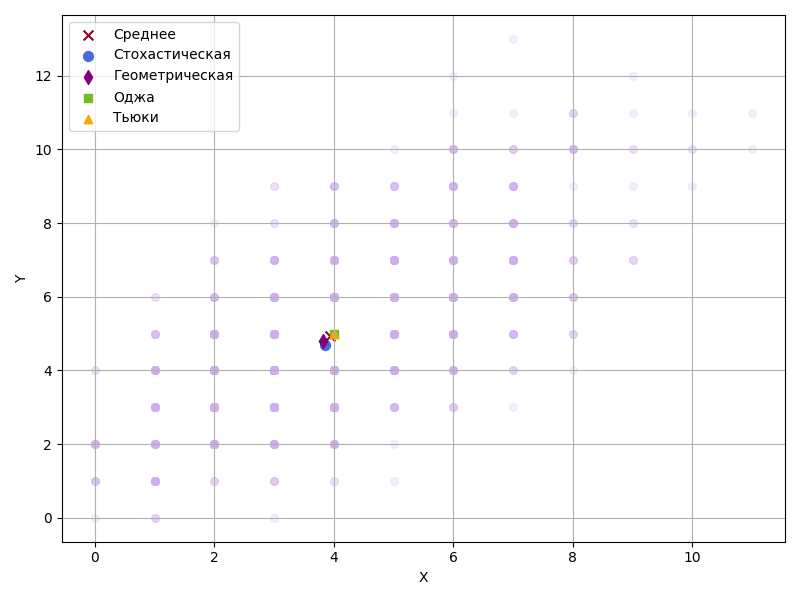
\includegraphics[width=0.9 \textwidth]{sample_poisson.png}
  \caption{Сравнение различных оценок многомерной медианы для дискретной выборки объема 1000 из двумерного распределения Пуассона с параметрами $\Lambda_{1}=4,\ \Lambda_{2}=5$. }
  \label{fig:poisson}
\end{figure}
\newpage

\subsubsection{Дискретное двумерное}

Рассмотрим теперь двумерное распределение следующего вида. Выборка генерируется как геометрическое распределение с параметром $p_1 = 0{,}5$ по первой оси и с параметром $p_2 = 0{,}2$ по второй. В этом случае математическое ожидание равно $(2; 5)^{\mathrm{T}}$.

Как видно из Рисунка~\ref{fig:geom}, только выборочное среднее совпадает с теоретическим математическим ожиданием. Остальные алгоритмы дают близкие между собой оценки, смещенные в одну сторону. Наибольшее смещение наблюдается у медианы Тьюки.

Вероятно, данное поведение связано с асимметрией распределения и дискретной природой выборки.
\newpage
\begin{figure}[!hhh]
   \centering
    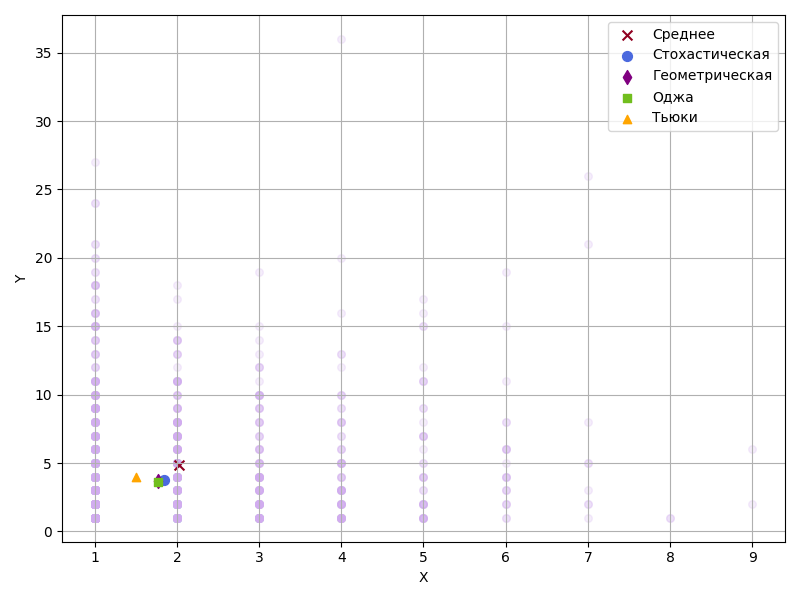
\includegraphics[width=0.95\textwidth]{sample_geom.png}
  \caption{Сравнение различных оценок многомерной медианы для дискретной выборки объема 1000, где распределение по каждой оси геометрическое с параметрами $p_1 = 0{,}5$ по первой оси и $p_2 = 0{,}2$ по второй.}
  \label{fig:geom}
\end{figure}

\vspace{2ex}

Таким образом, проведенные эксперименты показывают, что предложенный алгоритм демонстрирует устойчивое поведение для широкого класса распределений и областей. В большинстве рассмотренных примеров предложенный алгоритм дает оценки, сопоставимые с геометрической медианой, что согласуется с результатами предыдущих исследований.